% !TEX root = ../beamer.tex

\begin{frame}[t]
	\frametitle{Model-Driven Software Development}
	\begin{center}
	\begin{tikzpicture}[
		>=stealth,
		box/.style = {draw, minimum width = 3cm, minimum height = 1.1cm, align=center},
		node distance = 1cm and 0.5cm
		]
		\node[box, fill=pantone312!10!white] (model) {Model};
		\node[box, below = of model] (dsl) {Domain-Specific\\Language};
		\draw[<-] (model) -- node[right] (uses) {} (dsl);
		\node[box, right = 1.75cm of uses] (generator) {Generator};
		\node[box, right = of generator] (platforms) {Code for\\Platforms};
		\draw[->] (dsl) -| (generator);
		\draw[->] (model) -| (generator);
		\draw[->] (generator) -- (platforms);
	\end{tikzpicture}
	\end{center}
	\vfill
    
    \begin{itemize}
       \item Cross-platform approach
       \item Develop a model once, for multiple platforms
       \item Development on a higher level of abstraction
    \end{itemize}
\end{frame}

\begin{frame}[t]
    \frametitle{Starting Base of \MD}
    
    \begin{center}   
	    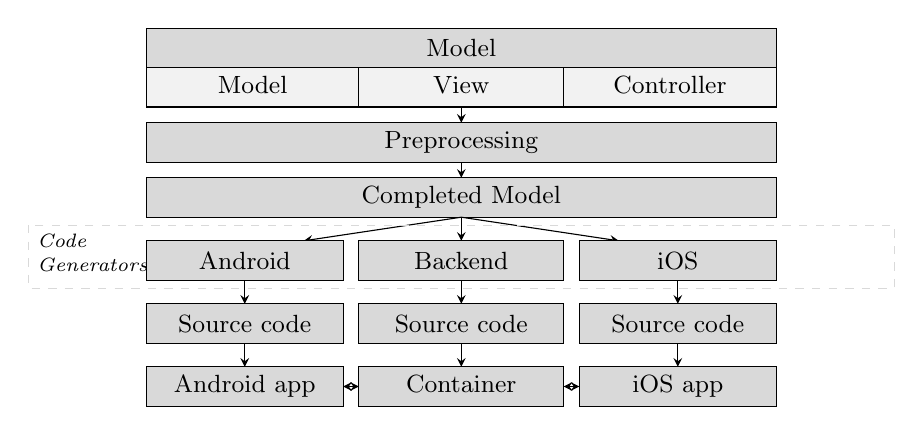
\begin{tikzpicture}[>=stealth]
		{\small
		    \draw [fill=gray!30!white] (-4,5) rectangle (4,5.5) node[pos=.5] {\MD Model};
		    \draw [fill=gray!10!white] (-4,4.5) rectangle (-1.3,5) node[pos=.5] {Model\vphantom{Aq}};
		    \draw [fill=gray!10!white] (-1.3,4.5) rectangle (1.3,5) node[pos=.5] {View\vphantom{Aq}};
		    \draw [fill=gray!10!white] (1.3,4.5) rectangle (4,5) node[pos=.5] {Controller\vphantom{Aq}};
		    
		    \draw [->] (0,4.5) -- (0,4.3);
		    
		    \draw [fill=gray!30!white] (-4,3.8) rectangle (4,4.3) node[pos=.5] {Preprocessing};
		    
		    \draw [->] (0,3.8) -- (0,3.6);
		    
		    \draw [fill=gray!30!white] (-4,3.1) rectangle (4,3.6) node[pos=.5] {Completed \MD Model};
		    
		    \draw [->] (0,3.1) -- (-2,2.8);
		    \draw [->] (0,3.1) -- (0,2.8);
		    \draw [->] (0,3.1) -- (2,2.8);
		    
		    \draw [gray!30!white, dashed] (-5.5,3) rectangle (5.5,2.2);
		    \node [right] at (-5.5,2.8) {\scriptsize{\textit{Code}}};
		    \node [right] at (-5.5,2.5) {\scriptsize{\textit{Generators}}};
		    		    
		    \draw [fill=gray!30!white] (-4,2.3) rectangle (-1.5,2.8) node[pos=.5] {Android};
		    \draw [fill=gray!30!white] (-1.3,2.3) rectangle (1.3,2.8) node[pos=.5] {Backend};
		    \draw [fill=gray!30!white] (1.5,2.3) rectangle (4,2.8) node[pos=.5] {iOS};
		    
		    \draw [->] (-2.75,2.3) -- (-2.75,2);
		    \draw [->] (0,2.3) -- (0,2);
		    \draw [->] (2.75,2.3) -- (2.75,2);
		    
		    \draw [fill=gray!30!white] (-4,1.5) rectangle (-1.5,2) node[pos=.5] {Source code};
		    \draw [fill=gray!30!white] (-1.3,1.5) rectangle (1.3,2) node[pos=.5] {Source code};
		    \draw [fill=gray!30!white] (1.5,1.5) rectangle (4,2) node[pos=.5] {Source code};
		    
		    \draw [->] (-2.75,1.5) -- (-2.75,1.2);
		    \draw [->] (0,1.5) -- (0,1.2);
		    \draw [->] (2.75,1.5) -- (2.75,1.2);
		    
		    \draw [fill=gray!30!white] (-4,0.7) rectangle (-1.5,1.2) node[pos=.5] {Android app\vphantom{Aq}};
		    \draw [fill=gray!30!white] (-1.3,0.7) rectangle (1.3,1.2) node[pos=.5] {Container\vphantom{Aq}};
		    \draw [fill=gray!30!white] (1.5,0.7) rectangle (4,1.2) node[pos=.5] {iOS app\vphantom{Aq}};	
		    
		    \draw [<->] (-1.5,0.95) -- (-1.3,0.95); 
		    \draw [<->] (1.5,0.95) -- (1.3,0.95);    
		}
	    \end{tikzpicture}
    \end{center}
{\hfill\color{gray}{\tiny{Source: \MD Project Seminar Presentation}}}

\end{frame}



\begin{frame}[t]
    \frametitle{Project Goals}
    
    \begin{itemize}
       \item Generate several apps from a single model
       \item Enable the specification of workflows between several apps
       \item The workflow specification should be simple, fast and easy to understand for programmers and customers
       \item Rough specification of a model should take no more than a few hours
       
    \end{itemize}
\end{frame}


